% !TEX encoding = UTF-8 Unicode
\documentclass[12pt]{article}
%\documentclass[12pt]{report}
\usepackage{color}
\usepackage{url}
\usepackage[T2A]{fontenc} % enable Cyrillic fonts
\usepackage[utf8]{inputenc} % make weird characters work
\usepackage{graphicx}

\usepackage[english,serbian]{babel}

\usepackage[unicode]{hyperref}
\hypersetup{colorlinks,citecolor=green,filecolor=green,linkcolor=blue,urlcolor=blue}

\usepackage{listings}

%\newtheorem{primer}{Пример}[section] %ćirilični primer
\newtheorem{primer}{Primer}[section]

\definecolor{mygreen}{rgb}{0,0.6,0}
\definecolor{mygray}{rgb}{0.5,0.5,0.5}
\definecolor{mymauve}{rgb}{0.58,0,0.82}

\lstset{ 
  backgroundcolor=\color{white},   % choose the background color; you must add \usepackage{color} or \usepackage{xcolor}; should come as last argument
          % the size of the fonts that are used for the code
  breakatwhitespace=false,         % sets if automatic breaks should only happen at whitespace
  breaklines=true,                 % sets automatic line breaking
  captionpos=b,                    % sets the caption-position to bottom
  commentstyle=\color{mygreen},    % comment style
  deletekeywords={...},            % if you want to delete keywords from the given language
  escapeinside={\%*}{*)},          % if you want to add LaTeX within your code
  extendedchars=true,              % lets you use non-ASCII characters; for 8-bits encodings only, does not work with UTF-8
  firstnumber=1,                % start line enumeration with line 1000
  frame=single,	                   % adds a frame around the code
  keepspaces=true,                 % keeps spaces in text, useful for keeping indentation of code (possibly needs columns=flexible)
  keywordstyle=\color{blue},       % keyword style
  language=Python,                 % the language of the code
  morekeywords={*,...},            % if you want to add more keywords to the set
  numbers=left,                    % where to put the line-numbers; possible values are (none, left, right)
  numbersep=5pt,                   % how far the line-numbers are from the code
  numberstyle=\tiny\color{mygray}, % the style that is used for the line-numbers
  rulecolor=\color{black},         % if not set, the frame-color may be changed on line-breaks within not-black text (e.g. comments (green here))
  showspaces=false,                % show spaces everywhere adding particular underscores; it overrides 'showstringspaces'
  showstringspaces=false,          % underline spaces within strings only
  showtabs=false,                  % show tabs within strings adding particular underscores
  stepnumber=2,                    % the step between two line-numbers. If it's 1, each line will be numbered
  stringstyle=\color{mymauve},     % string literal style
  tabsize=2,	                   % sets default tabsize to 2 spaces
  title=\lstname                   % show the filename of files included with \lstinputlisting; also try caption instead of title
}

\begin{document}

\title{Analiza '101 Innovations - Research Tools Survey' skupa podataka\\ \small{Seminarski rad u okviru kursa\\Istraživanje podataka 1\\ Matematički fakultet}}

\author{Dimitrije Antić\\ mi16128@alas.matf.bg.ac.rs}

\date{avgust 2019.}

\maketitle

\abstract{

U ovom radu su dati rezultati istraživanja skupa podataka \textit{101 Innovations - Research Tools Survey}. Nakon kratkog opisa strukture samog skupa, opisan je nacin na koji je on obrađen kako bi se prilagodio korišćenim alatima. Veliki broj informacija je dobijen kao izlaz iz određenih algoritama. Postupak analize podataka je opisan u daljem tekstu, a najbolje rezultate pri klasifikaciji je dala neuronska mreža.}

\tableofcontents

\newpage

\section{Opis skupa podataka}
\label{sec:opis skupa podataka}

\textit{101 Innovations - Research Tools Survey} je skup podataka koji sadrži informacije o online anketama koje su popunjavali korisnici, odgovarajući na pitanja o 17 istraživačkih aktivnosti. 20,663 ankete su popunjene u periodu od 10.5.2015. do 10.2.2016.

Sadrži 178 kolona, i 20663 instanci. Svaka od kolona je kategoričkog tipa, skup podataka ne sadrži ni jedan neprekidni atribut. Veliki broj kolona je binaran i predstavlja jedan od ponuđenih odgovora unapred zadatih u anketi. 

Takođe, u svakoj grupi ponuđenih odgovora postoji i odgovor \textit{eng. Other} koje ispitaniku daje mogućnost popunjavanja tzv. \textit{eng. open text} polja odnosno kolona u kojima ispitanik sam daje odgovor.

Ciljni atribut je atribut \textbf{eng. ROLE} koji predstavlja ulogu ispitanika, i inicijalno sadrži 8 različitih vrednosti.

Skup je u svojoj originalnoj formi organizovan u CSV format, u istoj formi je i korišćen u istraživanju. Oblik podataka je menjan u zavisnosti od korišćenog alata odnosno algoritma.

\section{Korišćeni alati}
Za obradu i analizu podataka korišćen je alat \textit{SPSS} i programski jezik \textit{Python} i pripadajuće biblioteke poput \textit{sklearn}, \textit{numpy}, \textit{pandas}, \textit{matplotlib}, \textit{keras} odnosno \textit{TensorFlow}.

Korišćena Jupyter sveska kao i \textit{tok podataka} korišćen u SPSS-u priloženi su uz rad.

\section{Preprocesiranje}	
\label{sec:preprocesiranje}

U ovom poglavlju ce biti objašnjen proces preprocesiranja, odnosno kako je skup podataka pripremljen za algoritme klasifikacije. 

Sam proces preprocesiranja vršen je u više koraka.

Jedan od koraka u preprocesiranju je predstavljao prevođenje odgovora iz tekstualnog oblika u broj, kako bi neuronska mreža na ulazu dobila vektore.

Odgovori su dati kao odvojeni kolone, ali mogu se organizovati u 17 grupa. Svaka od grupa predstavlja odgovor na jedno pitanje u vezi sa istraživanjima ispitanika. Tabela je data na sledećoj strani.

\newpage

\begin{table}
\label{tab:tabela}
\begin{center}
\caption{Kolone u skupu podataka}
\begin{tabular}{|c|c|} \hline
\textbf{Grupa atributa}& \textbf{Opis grupe atributa}\\ \hline
ROLE & ciljni atribut, uloga istraživača\\ \hline
ROLESPECCL & open text odgovor za ulogu istraživača \\ \hline
COUNTRYCL & open text odgovor za državu stanovanja \\ \hline
group\_1 & disciplina (nauka) kojom se bavi istraživač\\ \hline
PUBYEAR & interval godina prvog objavljenog rada\\ \hline
group\_2 & alat/sajt korišćen za pretragu literature\\ \hline
group\_3 & alat/sajt korišćen za pristup literaturi\\ \hline
group\_4 & alat/sajt korišćen za predloge literature\\ \hline
group\_5 & alat/sajt korišćen za pregledanje literature\\ \hline
group\_6 & alat/sajt korišćen za analiziranje podataka\\ \hline
group\_7 & alat/sajt korišćen za deljenje radova/protokola\\ \hline
group\_8 & alat/sajt korišćen za pripremu/pisanje radova\\ \hline
group\_9 & alat/sajt korišćen za organizaciju referenci\\ \hline
group\_10 & alat/sajt korišćen za arhiviranje radova\\ \hline
group\_11 & alat/sajt korišćen za arhiviranje/deljenje programskih kodova\\ \hline
group\_12 & alat/sajt korišćen za izbor časopisa za objavu rada\\ \hline
group\_13 & alat/sajt korišćen za objavljivanje radova\\ \hline
group\_14 & alat/sajt korišćen za edukaciju van akademskih aktivnosti\\ \hline
group\_15 & korišćeni istraživački profili\\ \hline
group\_16 & alat/sajt korišćen za pregledanje/recenziju radova\\ \hline
group\_17 & alat/sajt korišćen za merenje uticaja\\ \hline
\end{tabular}
\label{tab:tabela1}
\end{center}
\end{table}


Kako je nezanemarljiv broj ispitanika popunjavao \textit{eng. open text} polja, odlučeno je da se iz svakog od tih polja najbrojnija vrednost izvuče kao još jedna vrednost odnosno kolona zarad dobijanja dodatnih informacija. Kriterijum koji je utvrđen eksperimentalno: ako je broj pojavljivanja najbrojnije vrednosti veći od 10\% broja ljudi koji su popunjavali tu kolonu, vrednost je izvučena u suprotnom nije.

Jedna od kolona bila je \textit{PUBYEAR} i kao što je opisano u \ref{tab:tabela}, i bila je očigledni kandidat za prebacivanje u redni tip podataka, s obzirom da su intervali imali hronološku zavisnost. To se ekperimentalno i pokazalo kao dobro rešenje.

Ceo proces preprocesiranja je rađen u programskom jeziku \textit{Python}. U zavisnosti od algoritma i alata koji je korišćen, skup podataka je transformisan u ciljni oblik. 

Oblik podataka korišćen za rad je s obzirom na broj kolona prikazan u jupyter svesci, i predstavljao je:
\begin{enumerate}
    \item Za rad u alatu SPSS, skup podataka je sadržao kolone navedene u \ref{tab:tabela}, gde je svaka od kolona imala ceo broj različitih vrednosti odnosno kategorija.
    \item Za rad u jeziku Python, skup podataka je sadržao 309 kolona (retka matrica), koje su bile binarnog tipa, odnosno predstavljale su 1/NaN polja i davale odgovor da li je ispitanik potvrdio taj unapred zadati odgovor.
\end{enumerate}

\newpage
\section{Klasifikacija}
\label{klasifikacija}
Potrebno je klasifikovani istraživača u 8 inicijalnih klasa. Kako je navedeno u sekciji \ref{sec:preprocesiranje}, dodata je još jedna, deveta, kao posledica velikog broja popunjenih polja otvorenog teksta.
Za klasifikaciju datog skupa podataka korišćeni su, pored navedenih, algoritmi KNN, logistička regresija iz navedenih alata ali s obzirom na lošije rezultate neće biti prikazivani. Oni koji su prikazali najbolje rezultate dati su u nastavku:
\begin{itemize}
  \item Neuronska mreža u Python-u
  \item XGBoost u SPSS-u 
  \item C5.0 algoritam u SPSS-u
\end{itemize}

Najbolja preciznost je postignuta klasifikacijom korišćenjem neuronskih mreža, i iznosi 0.6224.

\subsection{Neuronske mreže}

Kako je skup podataka sam po sebi velike dimenzionalnosti, kod neuronskih mreža su dodavane određene modifikacije kako bi na što efikasniji način bilo sprečeno preprilagođavanje modela. 
Korišćena su unapređenja kao npr. \textit{eng. dropout rate} koji se zadaje verovatnoća sa kojim će se izlaz iz jednog neurona koristiti, odnosno verovatnoća sa kojom se rezultati neurona prihvataju.
Kao funkcija greške je korišćena srednje kvadratna greška.

Uz neuronsku mrežu iz biblioteke \textit{Keras}, korišćena je i \textit{eng. auto encoder} neuronska mreža koja je imala za zadatak smanjivanje dimenzionalnosti.

Eksperimenti su vršeni na više različitih oblika podataka dobijenih na načine opisane u u poglavlju \ref{sec:preprocesiranje}:
\begin{enumerate}
  \item Izvučene su nove kolone na osnovu slobodnih odgovora korisnika,
  \item Dodata nova klasa, u kombinaciji sa prethodnim oblikom,
  \item Nove kolone, nova klasa, sa atributom koji se odnosi na državu istraživača,
  \item Nove kolone, nova klasa, bez atributa koji se odnosi na državu istraživača.
\end{enumerate}

Najbolji rezultat je dobijen pri radu sa skupom podataka u obliku \textbf{3}, i to sledeće vrednosti:
\begin{itemize}
  \item \textbf{Bez autoencodera}: preciznost: 0.6224, greška: 1.2568
  \item \textbf{Sa autoencoderom}: preciznost: 0.6159, greška: 1.1670
\end{itemize}
\begin{center}
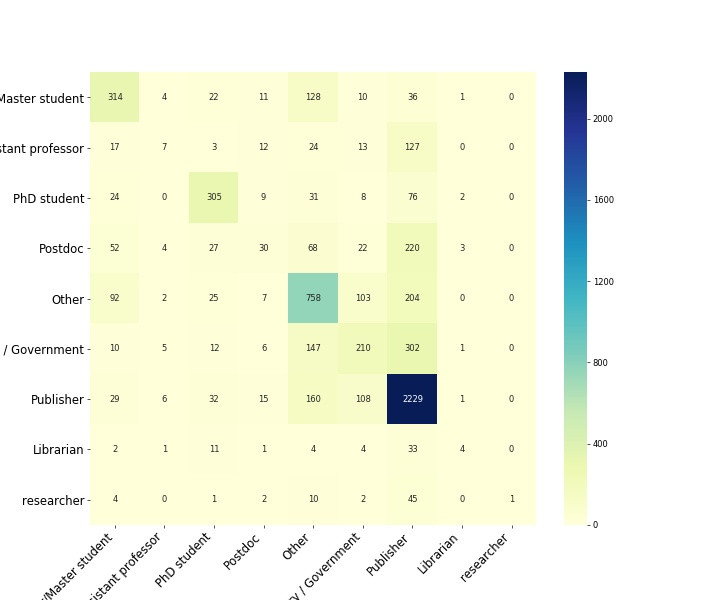
\includegraphics[width=1.1\textwidth, height=0.45\textheight]{fully_connected_conf_mat.jpg}
\caption{Matrica konfuzije neuronske mreže bez autoencodera}
\label{fig:figure1}
\end{center}
\begin{center}
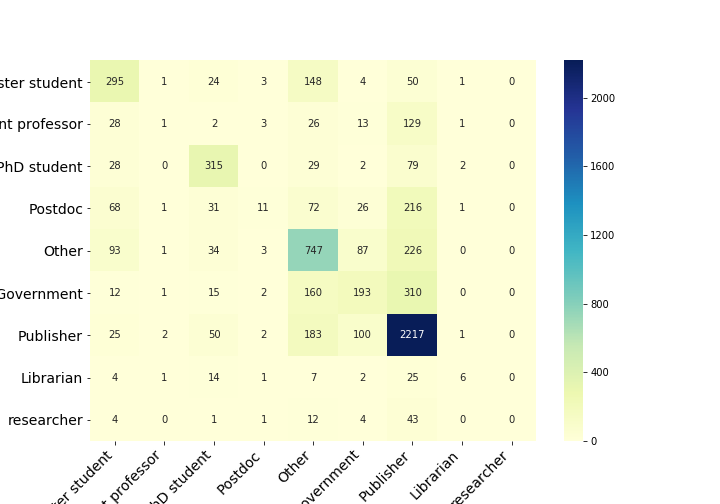
\includegraphics[width=1.1\textwidth, inner]{latent_fully_conf_mat.png}
\caption{Matrica konfuzije neuronske mreže sa autoencoderom}
\label{fig:figure2}
\end{center}
Iz matrica konfuzije mogu se izvesti zaključci koji se pojavljuju i kod drugih modela, zbog toga biće opisani samo jednom. Neuronska mreža je najpreciznije klasifikovala klasu Publisher, što je i očekivano s obzirom da je najbrojnija, pa je model bio dobro istreniran da je prepozna. Klasa Publisher se ujedno najviše meša i sa Industry/Government, Postdoc, Other, i Asisstant professor, što ima smisla jer je očekivano da su svi iz navedenih krugova sličniji Publisher-u nego npr Master student. Nova klasa nije doprinela preciznosti, ali potvrđuje prethodno navedeni zaključak, vrlo je očekivano od nekoga ko je researcher da ujedno i objavljuje radove.

\newpage

\subsection{XGBoost}

Za rad sa ovim algoritmom korišćen je alat \textit{SPSS} i odgovarajući oblik dat u poglavlju \ref{sec:preprocesiranje}. Predstavlja varijaciju Random forest ansambla koji koristi \textit{eng. gradient boosting} kako bi se još efikasnije sprečilo preprilagođavanje.

Rezultati klasifikacije korišćenjem \textit{XGBoost} klasifikatora su:

\begin{center}
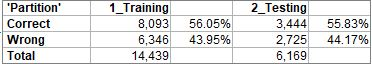
\includegraphics[width=0.8\textwidth]{xgboost_acc.JPG}
\caption{Preciznost algoritma}
\label{fig:figure4}
\end{center}
S obzirom na broj klasa i format matrice konfuzije dobijene iz alata SPSS, matrica neće biti prikazana u radu (zbog nemogućnosti prikazivanja na širini strane), i biće prikaza na odbrani rada.
Može se pogledati u \textit{eng. streamu} izvedenom iz SPSS-a.



\subsection{C5.0}

Za rad sa ovim algoritmom korišćen je alat \textit{SPSS} i odgovarajući oblik dat u poglavlju \ref{sec:preprocesiranje}.
Korišćen je algoritam C5.0 sa \textit{eng. boosting}-om, i ostvario sledeće rezultate:

\begin{center}
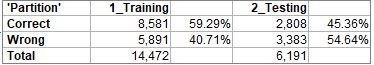
\includegraphics[width=0.8\textwidth]{C50_conf_matrix.JPG}
\caption{Preciznost na trening i test skupu}
\label{fig:figure3}
\end{center}

S obzirom na broj klasa i format matrice konfuzije dobijene iz alata SPSS, matrica neće biti prikazana u radu (zbog nemogućnosti prikazivanja na širini strane), i biće prikaza na odbrani rada.
Može se pogledati u \textit{eng. streamu} izvedenom iz SPSS-a.

\begin{center}
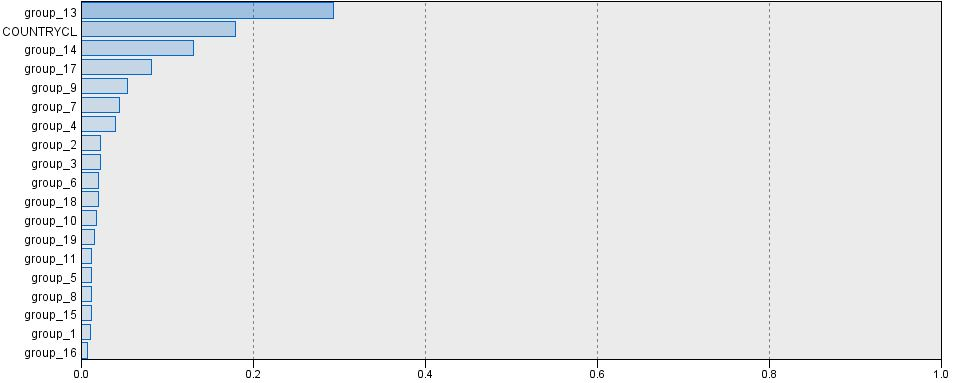
\includegraphics[width=1.2\textwidth]{c50_predictor.JPG}
\caption{Bitnost atributa korišćenih u klasifikaciji}
\label{fig:figure5}
\end{center}

Prehodni grafikon prikazuje bitnost atributa u procesu klasifikacije. Kao najbitniji se pokazao \textit{group\_13} koji prema opisu iz \ref{tab:tabela} govori o alatu koji se koristi za objavljivanje radova. Kako postoje osobe koje nisu istraživači koji objavljuju radove, za vrednost ovog polja su odgovarali sa \textit{Other}, a specijalno polje popunjavali vrednošću \textit{eng. none}. Pritom, ta vrednost nije izvedena kao nova kolona jer se ne uklapa u kriterijum naveden u poglavlju \ref{sec:preprocesiranje}.

Kao najmanje bitni:
\begin{itemize}
  \item \textit{group\_1} koji se odnosi na granu nauke u kojoj se istražuje, što je i očekivano jer se na osnovu nauke ne može jasno zaključiti da li je neko student, istraživač, profesor ili nešto drugo od navedenih klasa.
  \item \textit{group\_13} koji predstavlja alat koji se koristi za recenziju radova.
\end{itemize}
\newpage
\section{Zaključak}
\label{sec:zakljucak}

Dobijeni rezultati se oslanjaju na podskup skupa podataka uz dodate nove kolone koje su doprinele preciznosti klasifikatora i dodatu novu klasu. 

Skup podataka nije standardizovan, odnosno dajući ispitaniku mogućnost da popuni polja otvorenog odgovora gubi se na konzistentnosti tj. povećava se šansa da odgovori čine nepotpunu informaciju. Samim tim, proces preprocesiranja i klasifikacije podataka je postaje zahtevniji. Veliki problem je bila dimenzionalnost koja s obzirom na tip podataka nije mogla biti redukovana bez gubitka informacija, a doprinosila je preprilagođavanju modela. Dodatna preciznost bi možda bila postignuta detaljnijom obradom polja otvorenih odgovora.


\end{document}
